% Intended LaTeX compiler: xelatex
\documentclass[aspectratio=149,11pt,italian]{beamer}
\usepackage{graphicx}
\usepackage{longtable}
\usepackage{wrapfig}
\usepackage{rotating}
\usepackage[normalem]{ulem}
\usepackage{amsmath}
\usepackage{amssymb}
\usepackage{capt-of}
\usepackage{icomma}
\usepackage{hyperref}
\institute{Università di Siena}
\usepackage{localheader}
\usepackage{tikz}
\usepackage{booktabs,tabularx,tabularray}
\usepackage{setspace}
\usepackage{quoting}
\usepackage[italian]{babel}
\usepackage{fancybox}
\usepackage{tabularray}
\newcolumntype{R}{>{\raggedleft\arraybackslash}X}
\newcommand\EMTR{\text{EMTR}}
\newcommand{\sumt}[2]{\sum_{t=1}^{+\infty}\dfrac{#1}{\left(#2\right)^t}}
\NewDocumentCommand\nroot{O{n}m}{\sqrt[\leftroot{2}\scalebox{.8}{$#1$}]{#2}}
\usetheme{default}
\author{Massimo D'Antoni}
\date{2023-2024}
\title{La tassazione del risparmio}
\subtitle{Scienza delle Finanze}
\hypersetup{
 pdfauthor={Massimo D'Antoni},
 pdftitle={La tassazione del risparmio},
 pdflang={Italian}}
\begin{document}

\maketitle

%%%%%%%%%%%%%%%%%%%%%%%%%%%%%%%%%%%%%%%%%%%%%%%%%%%%%%%%%
\begin{frame}{Bisogna tassare i proventi del risparmio?}
Argomenti contrari:
\begin{itemize}
\item Argomento tradizionale: doppia tassazione del risparmio (J.S. Mill)
\item L'argomento "moderno": la tassazione del reddito da capitale distorce
l'allocazione intertemporale delle risorse (scoraggia il risparmio)
\begin{itemize}
\item ma quanto è "elastico" il risparmio rispetto al rendimento?
\end{itemize}
\item L'argomento pragmatico: la tassazione del reddito da capitale ha un gettito
effettivo vicino a zero perché tassa solo la componente \emph{riskless} del
rendimento di un investimento (vedi oltre)
\end{itemize}
Argomenti a favore:
\begin{itemize}
\item la possibilità di trasformare reddito da lavoro in reddito di capitale rende
necessario tassare il reddito di capitale
\item è un modo per tassare indirettamente i lasciti ereditari (penalizzare i
\emph{rentier}); rispetto a tassazione delle successioni (che è un'imposta
patrimoniale) la tassazione del capitale presenta dei vantaggi se c'è
eterogeneità dei rendimenti
\end{itemize}
\end{frame}

\section{Il trattamento fiscale del risparmio}

%%%%%%%%%%%%%%%%%%%%%%%%%%%%%%%%%%%%%%%%%%%%%%%%%%%%%%%%%
\begin{frame}{Classificiazioni e modalità di tassazione}
\begin{itemize}
\item La tassazione varia a seconda della tipologia di reddito:
\begin{itemize}
\item \alert{interessi}: ammontare e data di percezione certi (o quasi). Il debitore spesso può portarli in deduzione, tassazione in capo al creditore non comporta doppia tassazione. Sono tassati alla maturazione (vedi però \emph{zero coupon}) con l'applicazione di ritenute.
\item \alert{dividendi}: tassazione al momento della distribuzione. Tassazione generalmente più blanda degli interessi (eccetto che con «metodo classico»)
\item \alert{plusvalenze} (e «derivati»): ammontare incerto, possono dar luogo a minusvalenze. Tassazione alla realizzazione, solitamente con imposte proporzionali, senza ritenute.
\end{itemize}
\item Varia a seconda del veicolo di investimento:
\begin{itemize}
\item se nell'ambito di un fondo comune di investimento è interamente reddito di capitale
\item se nell'ambito di attività di impresa è reddito di impresa
\end{itemize}
\end{itemize}
\end{frame}

%%%%%%%%%%%%%%%%%%%%%%%%%%%%%%%%%%%%%%%%%%%%%%%%%%%%%%%%%
\begin{frame}{I tre momenti della tassazione}
Il risparmio può essere sottoposto a tassazione in tre momenti:
\begin{itemize}
\item accantonamento (una parte del reddito è investita)
\item accumulazione (l'investimento produce rendimenti)
\item prelievo (il capitale e relativi rendimenti sono disinvestiti)
\end{itemize}

\begin{figure}
\centering
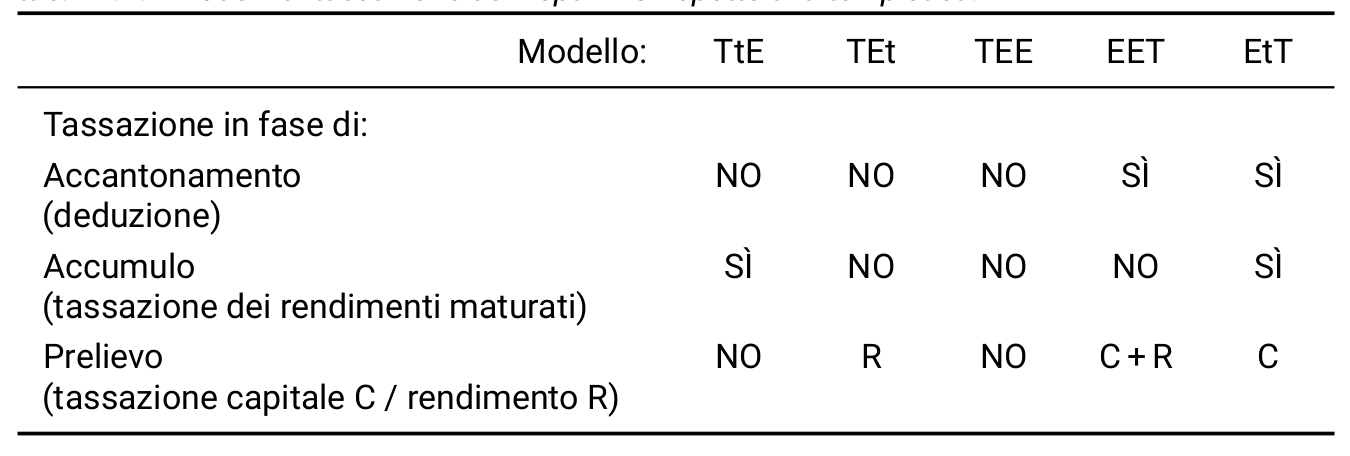
\includegraphics[width=\textwidth]{./figure/modelli-tassazione-risparmio.png}
\end{figure}
\end{frame}


%%%%%%%%%%%%%%%%%%%%%%%%%%%%%%%%%%%%%%%%%%%%%%%%%%%%%%%%%
\begin{frame}{I modelli di tassazione}
Vi sono diversi schemi di tassazione:
\begin{itemize}
\item \alert{TtE}: il reddito risparmiato ha pagato l'imposta e paga imposte sui
rendimenti. È il modello più diffuso in Italia e non solo: tassazione degli
interessi, conti correnti, conti titoli presso intermediario
\item \alert{TEt}: il reddito risparmiato ha pagato l'imposta, i rendimenti sono tassati
al momento della percezione da parte del titolare del fondo. Esempio:
plusvalenze, ma anche assicurazioni vita
\item \alert{TEE}: esenzione, si applica ai PIR (Piani individuali di risparmio), per
incentivare l'investimento in imprese italiane
\item \alert{EET}: esenzione da imposta al momento dell'accantonamento, nessuna
tassazione dei rendimenti, sono tassati i prelievi
\begin{itemize}
\item Esempio: fondi pensione americani (IRA) e fondi di risparmio britannici (ISA)
\item l'EET è equivalente al TEE
\end{itemize}
\item \alert{EtT}: previdenza complementare e TFR
\end{itemize}
\end{frame}

%%%%%%%%%%%%%%%%%%%%%%%%%%%%%%%%%%%%%%%%%%%%%%%%%%%%%%%%%
\begin{frame}{La tassazione del risparmio in Italia: le aliquote}
\begin{center}
\centering
\includegraphics[height=7cm]{./figure/aliquote-attività-finanziarie.png}
\end{center}
\end{frame}


%%%%%%%%%%%%%%%%%%%%%%%%%%%%%%%%%%%%%%%%%%%%%%%%%%%%%%%%%
\begin{frame}{La tassazione del risparmio in Italia: le modalità di prelievo}
Le modalità di prelievo variano a seconda della scelta del regime
\begin{itemize}
\item \alert{risparmio amministrato} (quando titoli in custodia ma non in gestione presso intermediario): l'intermediario applica l'imposta e compensa eventuali minusvalenze con plusvalenze nell'ambito dello stesso rapporto.
\item \alert{regime della dichiarazione} (se non c'è intermediazione o comunque a scelta del contribuente):  in sede Irpef indicazione analitica da parte del contribuente, che calcola e versa l'imposta sostitutiva; può compensare minusvalenze con altri redditi diversi;
\item \alert{risparmio gestito} (gestioni patrimoniali individuali o collettive previdenziali)
\item \alert{fondi comuni} (quando non detenuti in una gestione patrimoniale)
\end{itemize}
\end{frame}

%%%%%%%%%%%%%%%%%%%%%%%%%%%%%%%%%%%%%%%%%%%%%%%%%%%%%%%%%
\begin{frame}{La tassazione del risparmio in Italia/2}
\begin{itemize}
\item \alert{risparmio gestito} (gestioni patrimoniali individuali o collettive previdenziali): imposta applicata dal gestore sul risultato di gestione su base annua.
\begin{center}
   \begin{tabular}{ll}
   \multicolumn{2}{l}{Risultato di gestione $=$} \tabularnewline
  &  Valore patrimonio a fine periodo \tabularnewline
   & $\minus$ Valore patrimonio a inizio periodo \tabularnewline
   & $+$ Prelievi e proventi distribuiti \tabularnewline
   & $\minus$ Conferimenti e sottoscrizioni \tabularnewline
   & $\minus$ Redditi esenti. \tabularnewline
  \end{tabular}
\end{center}
Comporta tassazione delle plusvalenze alla maturazione e compensazione delle minusvalenze con redditi di capitale
\item \alert{fondo comune} in regime di risparmio amministrato o dichiarazione: tassazione in caso di distribuzione periodica o riscatto/liquidazione/cessione della quota.\\[0pt]
Implicitamente redditi di capitale e plusvalenze nell'ambito del fondo si compensano. Inoltre, vantaggio del differimento
\end{itemize}
\end{frame}

%%%%%%%%%%%%%%%%%%%%%%%%%%%%%%%%%%%%%%%%%%%%%%%%%%%%%%%%%
\begin{frame}{Piani individuali di risparmio}
Introdotti da L. Bilancio 2017, sono rivolti ai piccoli risparmiatori e
finalizzati all'investimento in imprese italiane di piccola e media
dimensione:
\begin{itemize}
\item rivolto a persone fisiche entro 30.000 di investimento annuale (150.000 complessivo)
\item investimenti per il 70\% in imprese italiane o europee con stabile
organizzazione in Italia
\item di tale 70\%, almeno il 30\% in imprese non rilevanti ai fini FTSE MIB
\item non più di 10\% nella stessa impresa o imprese dello stesso gruppo
\item strumenti finanziari tenuti in portafoglio per almeno 5 anni
\end{itemize}
Benefici fiscali:
\begin{itemize}
\item esenzione da imposte su redditi di capitale o diversi (in pratica, adozione
del modello TEE)
\end{itemize}
\end{frame}

%%%%%%%%%%%%%%%%%%%%%%%%%%%%%%%%%%%%%%%%%%%%%%%%%%%%%%%%%
\begin{frame}{Fondi pensione}
\begin{itemize}
\item Fondi pensione: minimo periodo contributivo di 5 anni, prestazione al
raggiungimento della pensione, almeno 50\% come rendita
\begin{itemize}
\item \alert{Fondi pensione chiusi}, costituiti sulla base di accordi negoziali fra i rappresentanti dei lavoratori e dei datori di lavoro
\item \alert{Fondi pensione aperti} istituite da banche, SGR, imprese d’investimento e imprese di assicurazione
\item \alert{Piani pensionistici individuali}, realizzate mediante contratti di assicurazione sulla vita e istituite da imprese di assicurazione
\end{itemize}
\item Trattamento fiscale:
\begin{itemize}
\item Prevista deducibilità IRPEF entro 5.164,57€/anno
\item Rendimenti tassati alla maturazione (risultato di gestione) al 20\%
\item Alla parte delle prestazioni che corrisponde ai contributi/premi versati
nella fase di accumulo si applica una tassazione separata, con un’aliquota
che dipende dagli anni di contribuzione: partendo dal 15\%, l’aliquota
viene ridotta di 0,3\% per ogni anno oltre il quindicesimo fino a un minimo
del 9\% (35 anni di contributi).
\item Su ulteriori rendimenti dopo il pensionamento aliquota del 26\%
\end{itemize}
\end{itemize}
\end{frame}

%%%%%%%%%%%%%%%%%%%%%%%%%%%%%%%%%%%%%%%%%%%%%%%%%%%%%%%%%
\begin{frame}{Regimi di tassazione delle pensioni in UE}
\begin{figure}
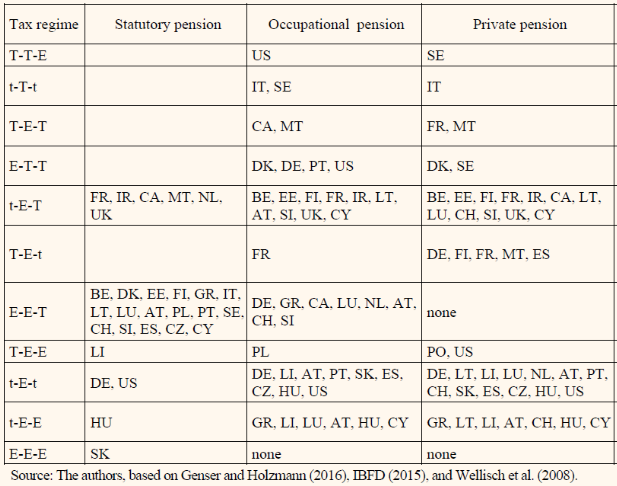
\includegraphics[width=.75\textwidth]{./figure/regimi-tassazione-pensioni.png}
\end{figure}
\end{frame}

%%%%%%%%%%%%%%%%%%%%%%%%%%%%%%%%%%%%%%%%%%%%%%%%%%%%%%%%%
\begin{frame}{TFR}
\begin{itemize}
\item L’impresa trattiene annualmente una quota della retribuzione pari circa a una mensilità. Al termine del rapporto di lavoro le trattenute rivalutate (a un tasso pari all’1,5\% più il 75\% dell’inflazione calcolata con l’indice
\end{itemize}
ISTAT) vengono corrisposte al lavoratore in un’unica soluzione.
\begin{itemize}
\item Trattamento fiscale (modello EtT)
\begin{itemize}
\item Somma accantonata interamente dedotta dall'IRPEF
\item Sulle rivalutazioni l’impresa applica un’imposta sostitutiva del 17\%, prelevata
\end{itemize}
\end{itemize}
alla maturazione.
\begin{itemize}
\item Al momento della cessazione del rapporto di lavoro la parte di capitale che rappresenta i rendimenti sarà esente perché già tassata.
\item La parte rimanente, che rappresenta il totale degli accantonamenti, viene assog-
\end{itemize}
getta all’IRPEF ma separatamente, con aliquota pari alla media delle aliquote
medie IRPEF degli ultimi 5 anni.
\end{frame}


%%%%%%%%%%%%%%%%%%%%%%%%%%%%%%%%%%%%%%%%%%%%%%%%%%%%%%%%%
\begin{frame}{La tassazione del risparmio in Italia: sintesi}
\begin{figure}
\centering
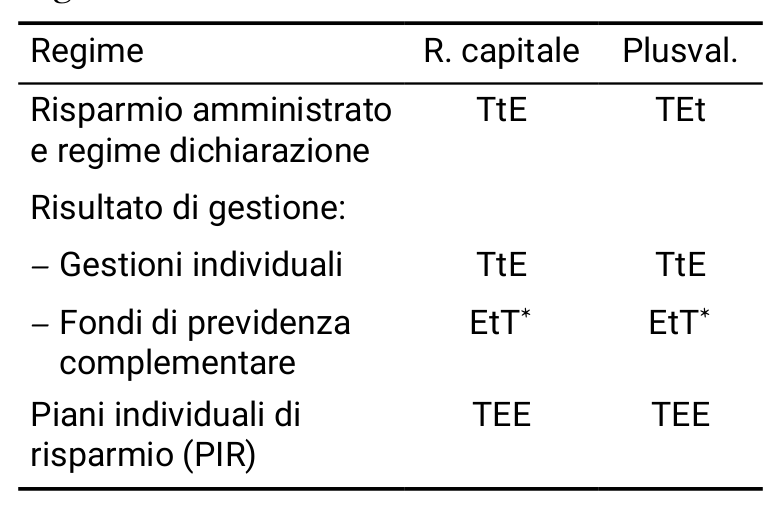
\includegraphics[height=6cm]{./figure/regimi-tassazione-risparmio-in-Italia.png}
\end{figure}
\end{frame}


%%%%%%%%%%%%%%%%%%%%%%%%%%%%%%%%%%%%%%%%%%%%%%%%%%%%%%%%%
\begin{frame}{I vari modelli di tassazione e la ricchezza finale netta}
\begin{itemize}
\item In assenza di imposte, un euro investito per $n$ periodi fornisce una
ricchezza finale pari a: $W_L=(1+R)^n$
\item Nel modello TtE la ricchezza netta finale è pari a: $W_N=(1+R(1-t))^n$
\item Nel modello TEt, la tassazione dei rendimenti è al momento del prelievo:
$$W_N=W_L-t(W_L-1)=W_L(1-t)+t=(1+R)^n(1-t)+t$$
\item Nel modello TEE: $W_N=(1+R)^n$
\item Nel modello EET: rinunciare a un euro per risparmiarlo signifia poter
investire $1/(1-t_p)$, dove $t_p$ è l'imposta sul reddito. Alla fine:
$$W_N=\frac{(1+R)^n}{1-t_p}(1-t_p)=(1+R)^n$$
\end{itemize}
\end{frame}

%%%%%%%%%%%%%%%%%%%%%%%%%%%%%%%%%%%%%%%%%%%%%%%%%%%%%%%%%
\begin{frame}{Confronto tra TtE e TEt}
\begin{figure}
\centering
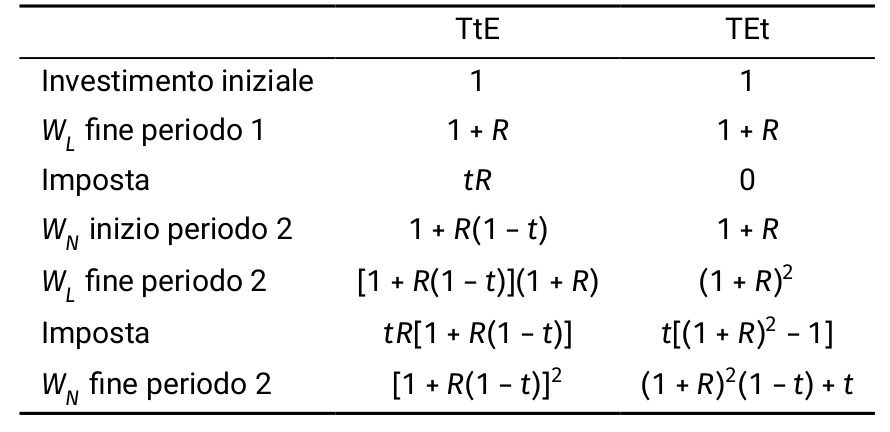
\includegraphics[height=5cm]{./figure/confronto-TtE-TEt.png}
\end{figure}

\begin{itemize}
\item Tte = maturazione, TEt = realizzazione
\item A parità di aliquota, una tassazione alla realizzazione risulta più
conveniente di una tassazione alla maturazione
\begin{itemize}
\item il vantaggio in termini di ricchezza netta finale è pari a $(tr)R(1-t)$
\end{itemize}
\end{itemize}
\end{frame}

%%%%%%%%%%%%%%%%%%%%%%%%%%%%%%%%%%%%%%%%%%%%%%%%%%%%%%%%%
\begin{frame}{Tassazione delle plusvalenze alla realizzazione o alla maturazione}
\begin{center}
\begin{tabular}{lrrrr}
 & 0 & 1 & 2 & 3\\[0pt]
\hline
Valore asset & 1000 & 1100 & 1250 & 1400\\[0pt]
Plusvalenza maturata &  & 100 & 150 & 150\\[0pt]
Plusvalenza realizzata &  &  &  & 400\\[0pt]
Imposta 20\% maturazione &  & 20 & 30 & 30\\[0pt]
Imposta 20\% realizzazione &  &  &  & 80\\[0pt]
\end{tabular}
\end{center}

\begin{itemize}
\item L'imposizione totale è la stessa nei due casi, ma la tempistica è diversa.
\item Il valore capitalizzato (al 10\%) dell'imposta alla maturazione è: 87,2,
maggiore di 80.
\end{itemize}
\end{frame}

%%%%%%%%%%%%%%%%%%%%%%%%%%%%%%%%%%%%%%%%%%%%%%%%%%%%%%%%%
\begin{frame}{L'aliquota effettiva associata ai diversi modelli di tassazione}
\begin{itemize}
\item Misuriamo l'aliquota effettiva è $(R-r)/R$ dove:
\begin{itemize}
\item $R =\nroot{W_L}-1$
\item $r=\nroot{W_N}-1$
\end{itemize}
\end{itemize}

\begin{figure}
\centering
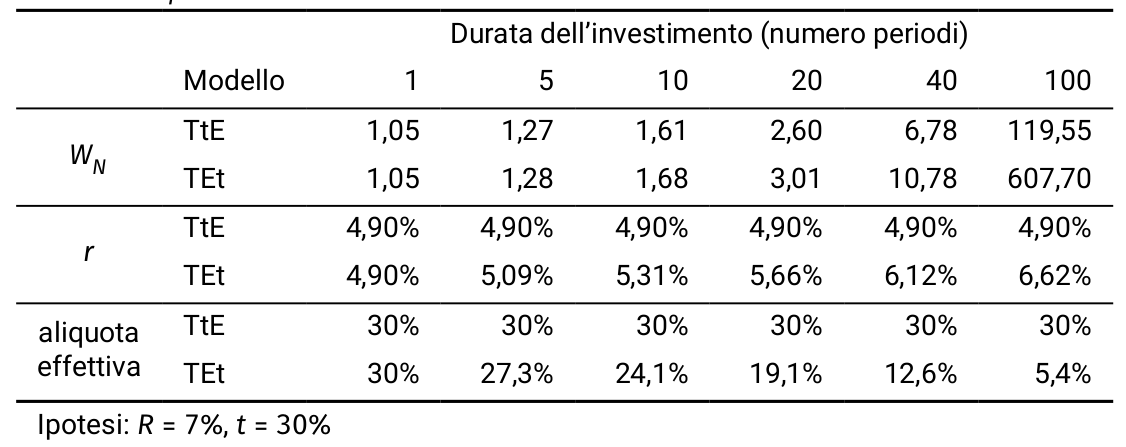
\includegraphics[width=\textwidth]{./figure/confronto-TtE-TEt-lungo-termine.png}
\end{figure}

\begin{itemize}
\item Nota Bene: il vantaggio diventa molto rilevante se l'orizzonte è molto lungo
\end{itemize}
\end{frame}



%%%%%%%%%%%%%%%%%%%%%%%%%%%%%%%%%%%%%%%%%%%%%%%%%%%%%%%%%
\begin{frame}{Tassazione alla realizzazione e \emph{lock-in}}
\begin{itemize}
\item Titolo acquistato a 100, in $t$ vale 200;
\item imposta su plusvalenze $g=20\%$
\item prevediamo che in $t+1$ il valore del titolo sarà aumentato di un ulteriore 6\%.
\item Confrontiamom due possibilità:
  \begin{description}
  \item[{Opzione 1}] Liquidare il titolo e acquistarne un altro. Pagniamo
    un'imposta di 20, reinvesto 180, rivendo il titolo a 190,8, pago imposta
    di $0,2\times(190,8-180)=2,16$, consumo 188,64
  \item[{Opzione 2}] Mantenere il titolo in portafoglio. Vendo il titolo a
    212, pago imposta $0,2\times(212-180)=22,4$, consumo 189,6
  \end{description}
\item Conviene l'opzione 2. Converrebbe anche se il rendimento ottenibile dal
  titolo alternativo fosse superiore al 6\% (es. 6,5\%).
\end{itemize}
La tassazione alla realizzazione incentiva a non modificare il portafoglio
corrente
\alert{anche in presenza di opportunità di investimento più convenienti}.\\
Si determina cioè \alert{un'allocazione inefficiente delle risorse}.
\end{frame}

\section{Tassazione della ricchezza}

%%%%%%%%%%%%%%%%%%%%%%%%%%%%%%%%%%%%%%%%%%%%%%%%%%%%%%%%%
\begin{frame}{Capitalizzazione di un'imposta}
\begin{itemize}
\item C'è equivalenza tra tassazione della ricchezza e tassazione del reddito da
capitale se questo è fisso
\begin{itemize}
\item Un'attività che dà un rendimento perpetuo di 10€ al tasso del 5\% vale:
10€/0,05=200€
\item Un'imposta del 20\% sul rendimento (rendimento netto 8€) produce una
riduzione una tantum del 20\% nel valore patrimoniale: l'imposta futura
viene capitalizzata
\item si noti che se il rendimento degli impieghi alternativi del capitale resta
al 5\% (cioè se non è stato a sua volta ridotto da analoga imposta), allora
il valore di mercato di un'attività che dà un rendimento netto di 8€ è
pari a 160€
\end{itemize}
\item Cioè: l'imposta sul rendimento dell'attività si traduce in una variazione
del valore di questa, che ricade su chi la detiene al momento
dell'introduzione dell'imposta
\item i successivi detentori dell'attività versano l'imposta ma in effetti non ne
pagano il costo, visto che l'imposta è stata scontata nel valore d'acquisto
\end{itemize}
\end{frame}

%%%%%%%%%%%%%%%%%%%%%%%%%%%%%%%%%%%%%%%%%%%%%%%%%%%%%%%%%
\begin{frame}{Tassazione della ricchezza o del reddito da capitale?}
\begin{itemize}
\item C'è equivalenza tra un'imposta sulla ricchezza e un'imposta sul
rendimento. Ipotizzando che le imposte siano in entrambi i casi applicate ex
post: $$ (1-\tau)(1+R)=1+R(1-t) \quad\implies\quad t=\tau\frac{1+R}{R}$$
\item L'equivalenza è meno ovvia se i rendimenti sono incerti.
Un'imposta sulla ricchezza, in quanto indipendente dall'esito di un
investimento rischioso, è un'imposta sul rendimento \emph{risk-free}
\item Dunque: l'imposta sulla ricchezza premia gli impieghi più rischiosi e
l'imposta sul reddito li penalizza?
\begin{itemize}
\item in realtà non è affatto ovvio che sia così: se l'individuo reagisce all'imposta sul
reddito aumentando l'esposizione al rischio, l'effetto dell'imposta sul
rischio viene interamente neutralizzato
\end{itemize}
\item L'equivalenza c'è se rendimento uniforme tra diverse attività
patrimoniali. Se rendimento differenziato l'imposta patrimoniale
"premia" (= tassa meno pesantemente rispetto a tassazione sul reddito) le
attività che danno rendimento più alto
\end{itemize}
\end{frame}

%%%%%%%%%%%%%%%%%%%%%%%%%%%%%%%%%%%%%%%%%%%%%%%%%%%%%%%%%
\begin{frame}{Tassazione della ricchezza nei paesi OCSE}
\begin{center}
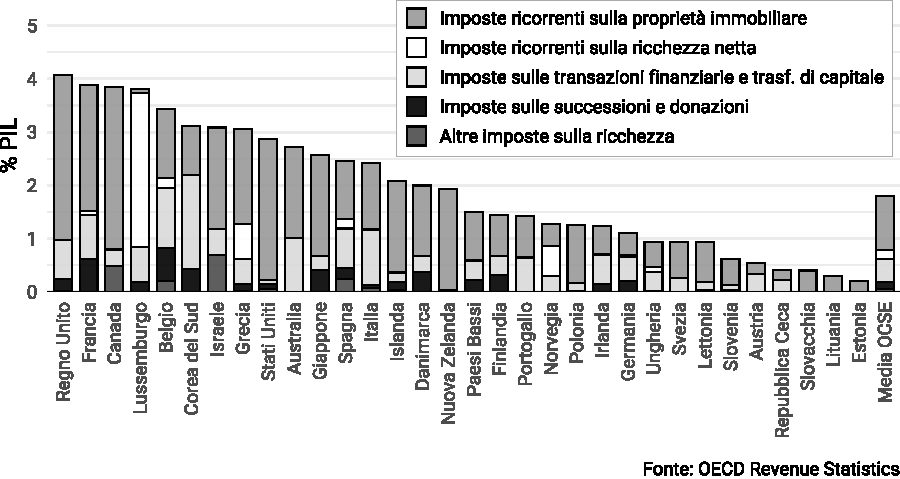
\includegraphics[width=\textwidth]{./figure/imposte-sulla-ricchezza-ocse.pdf}
\end{center}
\end{frame}

%%%%%%%%%%%%%%%%%%%%%%%%%%%%%%%%%%%%%%%%%%%%%%%%%%%%%%%%%
\begin{frame}{Tassazione della ricchezza}
\begin{itemize}
\item Tassazione sul possesso di ricchezza (tipicamente \emph{ricchezza netta} =
ricchezza al netto dei debiti)
\begin{itemize}
\item straordinarie (\emph{una tantum})
\item ordinarie (applicate annualmente)
\end{itemize}
\item Tassazione sul trasferimento di ricchezza (successione, donazioni, imposte di registro)
\item Ricorre la proposta di un'imposta personale sulla ricchezza (progressiva, con esenzione)
\begin{itemize}
\item in Europa esista in Svizzera, Norvegia e Spagna (la Francia l'ha abolita
nel 2018, altri paesi che avevano questa imposta l'hanno abbandonata)
\item prevede una soglia di esenzione
\item categorie di ricchezza solitamente esenti: abitazione principale,
patrimonio delle piccole imprese, ricchezza pensionstica\ldots{} esente
ovviamente il capitale umano
\item scarso gettito, costi elevati di amministrazione, rischio di fuga di
capitali, difficoltà di valutazione di alcuni cespiti
\end{itemize}
\end{itemize}
\end{frame}



%%%%%%%%%%%%%%%%%%%%%%%%%%%%%%%%%%%%%%%%%%%%%%%%%%%%%%%%%
\begin{frame}{Le imposte patrimoniali in italia}
\begin{itemize}
\item Imposte sulla ricchezza immobiliare:
\begin{itemize}
\item IMU, Imposta Municipale Unica.
Base imponibile: la rendita catastale x
coefficiente (160 per immobili a uso residenziale).\\[0pt]
Aliquota: 0,76\%, il
Comune può aumentarla o ridurla fino a 0,3\%.\\[0pt]
Esenzione: le abitazioni principali
\item IVIE per immobili ubicati all'estero
\item Imposte di registro, ipotecarie e catastali
\end{itemize}
\item Imposte sulla ricchezza finanziaria:
\begin{itemize}
\item \alert{Imposta di bollo} dello 0,2\% sui titoli detenuti in Italia; di 34,20
€/anno (100 €/anno per imprese) su conti correnti con giacenza media $\ge$ 5.000 €
\item analoga imposta sulle attività finanziarie detenute all'estero (\alert{Ivafe})
\item imposta sul trasferimenti della proprietà di azioni e altri strumenti
finanziari (\alert{Tobin Tax}) con un'aliquota dello 0,2\%, ridotta a 0,1\% se in mercati
regolamentati.
\end{itemize}
\item Imposte di successione: aliquota del 4\% sulla somma ereditata che eccede il
milione di € (per erede)
\end{itemize}
\end{frame}
\end{document}